\documentclass{article}

\usepackage[preprint]{neurips_2025}

\usepackage[utf8]{inputenc}
\usepackage[T1]{fontenc}
\usepackage{hyperref}
\usepackage{url}
\usepackage{booktabs}
\usepackage{amsfonts}
\usepackage{amsmath}
\usepackage{graphicx}
\usepackage{natbib}
\usepackage{microtype}
\usepackage{placeins}

\title{OATH: Quantifying Video Hallucination via Occlusion Debt}

\author{Anonymous Authors}

\begin{document}

\maketitle

\begin{abstract}
Video generators often produce clips that look realistic frame by frame while violating object permanence, temporal continuity, and implied world state, leaving a gap between visual quality and actual temporal reliability \cite{vbench2024,fvd2018,clipscore2021,tifa2023}. Existing evaluation practice emphasizes perceptual realism, prompt alignment, or internal uncertainty, but these signals do not directly measure whether entities and scene state persist coherently through occlusion and transition \cite{vbench2024,t2vcompbench2024,dreamdojo2026,fideseq2024}. We introduce \textbf{OATH} (Occlusion-Aware Temporal Hallucination), a persistence-centered metric that quantifies hallucination as \textbf{occlusion debt}, the mismatch between continuity that a video establishes before an occlusion and what it shows afterward. OATH combines occlusion-aware persistence estimation, identity-free matching, and reliability-aware aggregation so that continuity can be evaluated without assuming perfect object identities, and on the reported benchmark tables the strongest variant attains a primary error of \textbf{0.1714}, compared with \textbf{0.2393} for a CLIP-temporal baseline and \textbf{1.6357} for a realism-only proxy; however, among the available paired tests, only the comparison showing Single-Factor Hallucination Profile worse than CLIP-T is statistically significant (\(p=0.0248\)), while favorable OATH-versus-CLIP-T differences are not accompanied by reported p-values. These results support a benchmark-specific conclusion: persistence-aware scoring is the most competitive family in the reported ranking, indicating that video hallucination is more usefully characterized by temporal persistence failure than by frame realism alone.
\end{abstract}

\section{Introduction}

Recent progress in text-to-video generation has made short clips dramatically more realistic, but realism alone has not solved hallucination. Generated videos can preserve texture, color, and lighting while still violating the logic of the scene: an object disappears after a brief occlusion, a moving entity reappears with inconsistent state, or a scene evolves in a way that no longer matches the world state the clip had already established. Such failures matter because they undermine the reliability of generated video in downstream settings that depend on continuity rather than only appearance, including temporal reasoning, robotics simulation, embodied planning, and video-as-world-model evaluation \cite{dreamdojo2026,genie2024,sora2024,videopoet2024,worldsim2024}. This distinction has become sharper as video models have improved on conventional perceptual benchmarks such as FVD and realism-oriented quality measures while continuing to exhibit failures of object permanence and causal continuity that remain obvious to human viewers \cite{fvd2018,vbench2024,t2vcompbench2024,videoscore2024}. In that sense, the central problem is no longer merely whether a generated frame looks plausible in isolation, but whether a generated sequence preserves an internally coherent world through time.

\begin{figure}[htbp]
    \centering
    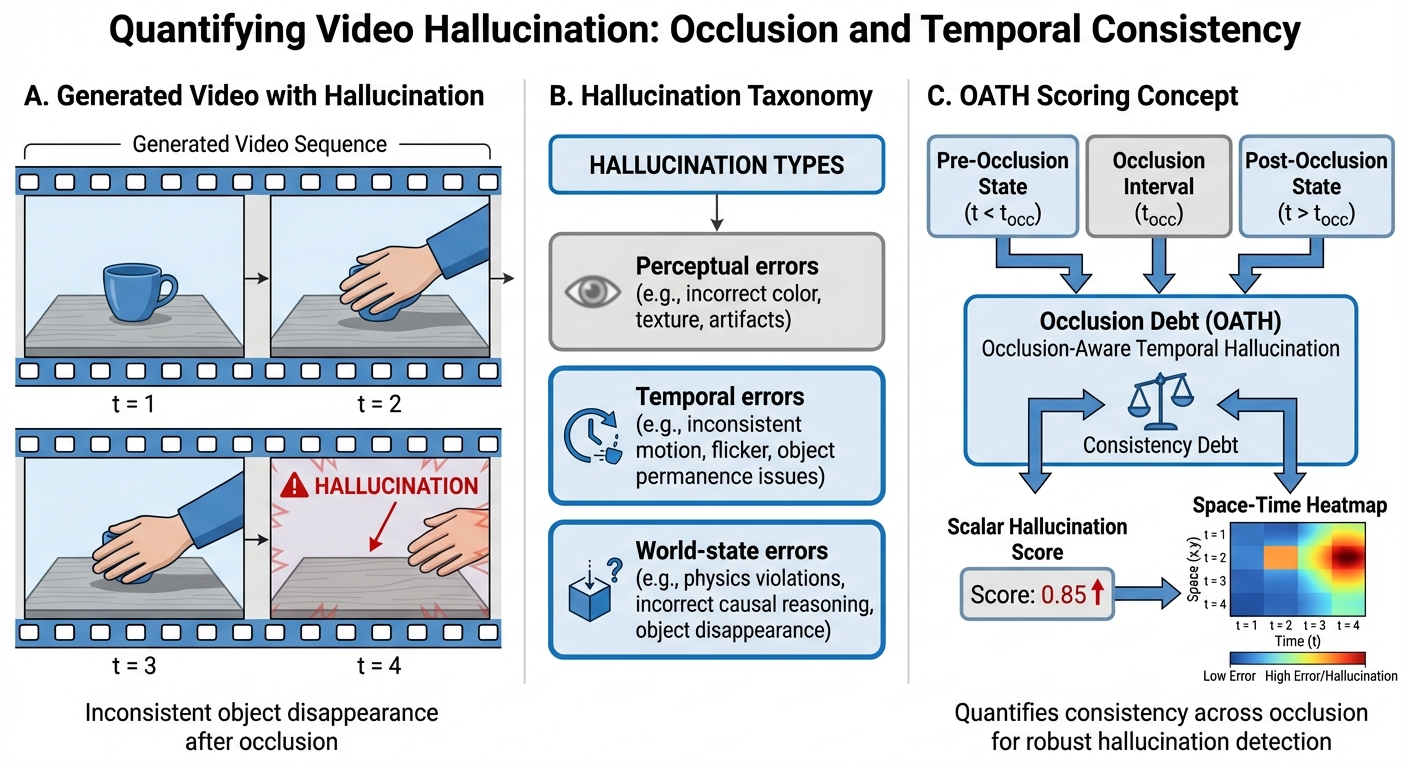
\includegraphics[width=0.85\textwidth]{figures/teaser_oath_hallucination_concept.png}
    \caption{Realistic frames can still hallucinate: OATH measures temporal persistence failures through occlusion debt.}
    \label{fig:teaser_oath_hallucination_concept}
\end{figure}

Existing evaluation paradigms are not designed for this failure mode. Perceptual metrics emphasize image sharpness, naturalness, and distributional similarity, which are useful when the main concern is artifacting or frame-level fidelity \cite{fvd2018,fideseq2024,vbench2024}. Prompt-alignment metrics instead ask whether a clip matches its text condition or retains descriptive similarity across neighboring frames, often using CLIP-derived similarity or instruction-following evaluators \cite{clipscore2021,clip2021,tifa2023,pickscore2023,blip2_2023}. Internal uncertainty signals and refinement diagnostics provide a third perspective by measuring instability during sampling or denoising \cite{videocrafter2024,consistency_models2023,diffusion_uncertainty2024}. Each family captures an important aspect of generation quality, yet none directly encodes the obligation that visible entities and scene state should persist coherently across time once the video has already established them. In practice, that gap is consequential: a metric can reward realism or coarse semantic alignment while ignoring a continuity failure that makes the clip unusable for tasks requiring state persistence, an issue that has also surfaced in recent discussions of evaluating foundation world models rather than purely generative media systems \cite{dreamdojo2026,genie2024,worldsim2024,egoworld2024}.

Building on this observation, we frame video hallucination as \textbf{temporal-world inconsistency under occlusion and transition}. The core idea is simple. Whenever a video establishes evidence that an entity or scene element should persist, the generator incurs an obligation to maintain that evidence when visibility changes. Hallucination is then the unpaid part of that obligation, which we call \textbf{occlusion debt}. This formulation yields \textbf{OATH} (Occlusion-Aware Temporal Hallucination), a metric that accumulates penalties when post-occlusion evidence fails to match expected continuity. Two design choices make the metric practical. First, OATH uses \textbf{identity-free matching}, which allows persistence to be evaluated without assuming perfect instance identity labels, an important property because generated videos often preserve category-level continuity while drifting in instance assignment. Second, OATH can incorporate \textbf{tracker reliability weighting} so that noisy track fragments do not dominate the score. Rather than treating hallucination as a broad aggregate of realism, semantics, and uncertainty, OATH focuses on the temporal persistence failures that the reported benchmark ranking places at the top of the evaluated methods. This design is also consistent with prior work on tracking, segmentation, and video-language alignment, which has shown that temporal evaluation becomes more robust when spatial correspondence and semantic evidence are used jointly rather than independently \cite{deepsort2017,bytetrack2022,sam2023,xmem2022,clip2021}.

The empirical pattern reported in the benchmark tables is consistent at the level of ranking even though formal significance evidence is incomplete. The three strongest primary-metric results all come from occlusion-debt variants, uncertainty-based methods are competitive but weaker on permanence alignment, long-horizon world consistency remains a strong baseline, and realism-only or broad composite methods perform substantially worse. This ranking sharpens the conceptual story of the paper: on this benchmark, hallucination in generated video is not primarily a perceptual-quality problem, and it is not fully captured by internal instability alone. Instead, the most useful signal is whether the generated world continues to make sense when temporal continuity is stressed by occlusion, motion, and state change. Our contributions are therefore fourfold:
\begin{itemize}
    \item We introduce a persistence-centered formulation of video hallucination that treats hallucination as \textbf{occlusion debt} accumulated across temporal transitions.
    \item We propose \textbf{OATH}, a practical metric with identity-free matching and reliability-aware aggregation for quantifying temporal permanence failures in generated videos.
    \item We present a comparative study over 19 reported evaluation conditions spanning realism proxies, semantic-faithfulness baselines, uncertainty-only methods, long-horizon consistency predictors, and targeted ablations.
    \item We show that permanence- and occlusion-aware scoring is the strongest method family in the reported benchmark ranking, while noting in the statistical analysis that only one provided paired comparison reaches \(p<0.05\) and that several favorable OATH comparisons are reported without p-values.
\end{itemize}

The rest of the paper develops this argument in stages. Section 2 reviews prior approaches to video evaluation and situates hallucination at the intersection of perceptual quality, semantic alignment, uncertainty, and world consistency. Section 3 then formalizes occlusion debt and describes the OATH metric in detail, including identity-free matching and reliability weighting. Section 4 describes the experimental protocol and benchmark organization used for the comparative analysis, after which Section 5 presents the main results and their statistical interpretation. Section 6 discusses what the ranking implies about how hallucination should be measured in generated video, and Section 7 consolidates concrete limitations. The resulting message is narrow but actionable: if the goal is to quantify hallucination in generated video, the strongest starting point in the reported evidence is to measure whether the generated world persists coherently through time.

\section{Related Work}

\subsection{Perceptual realism and video-quality evaluation}

A substantial literature evaluates generated video through perceptual realism, asking whether clips are sharp, stable, and visually plausible to human observers or to pretrained recognition features \cite{fvd2018,vbench2024,videoscore2024,fideseq2024,imagenvideo2022,makeavideo2022}. This tradition is important because low-level artifacts, flicker, unstable textures, and motion blur remain common failure modes in generative systems, and metrics such as FVD have become standard summaries of overall sample quality \cite{fvd2018,imagenvideo2022,makeavideo2022}. More recent benchmarking efforts extend this perspective by combining aesthetic quality, motion smoothness, subject consistency, and other perceptual subdimensions into broader evaluation suites \cite{vbench2024,t2vcompbench2024}. These metrics are useful for comparing generators as visual media systems, but their strength is also their limitation for hallucination analysis. By compressing evaluation into plausibility or realism, they can rate a temporally inconsistent but photorealistic clip too highly if the local pixels remain convincing. Our work differs from this realism-first perspective by treating continuity breakdown, rather than appearance degradation, as the primary object of measurement.

This distinction has become more important as modern generators have improved enough that many failures are no longer obviously visible in single frames. A clip can look polished and still break object permanence, causal consequences, or state continuity across occlusion \cite{sora2024,videogpt2021,worldsim2024}. In such settings, frame-level realism becomes a weak surrogate for whether the sequence encodes a coherent world. That mismatch is reflected in the reported benchmark ranking, where the realism-only proxy is among the weakest conditions. In contrast to perceptual quality metrics, OATH asks whether the entities and scene elements that the video has already established continue to behave as though they belong to the same underlying world. This places the method closer to temporal verification than to aesthetic evaluation.

\subsection{Prompt alignment, semantic faithfulness, and video-language metrics}

A second family of methods evaluates whether a generated clip matches its conditioning signal, typically a text prompt or task instruction \cite{clip2021,clipscore2021,tifa2023,pickscore2023,blip2_2023,instructblip2023}. In text-to-video settings, these approaches are attractive because they connect evaluation to intended content rather than to generic realism. A model that generates the wrong object, action, or scene can be penalized even if the result is visually plausible \cite{videopoet2024,modelscope_t2v2023,zeroscope2023}. Temporal extensions of prompt-faithfulness also attempt to assess whether neighboring frames remain semantically coherent over time, often by aggregating CLIP-like similarity across frames or across clips \cite{clip2021,clipscore2021,videoscore2024,t2vcompbench2024}. This improves over static prompt matching and captures a portion of temporal quality.

Even so, prompt alignment does not directly encode object permanence or delayed causal consistency. A video can remain semantically similar to its prompt while hallucinating key temporal events. A prompt may specify ``a dog running behind a sofa and reappearing,'' and a generated clip may depict a dog and a sofa in every frame while still failing to preserve the dog's continuity through the occlusion. That error is not, in the usual sense, a prompt mismatch; it is a world-state inconsistency. The reported results support this distinction. CLIP-T is competitive relative to some weaker controls, but it does not match the best occlusion-debt variants in the primary ranking. OATH differs from prompt-alignment metrics by evaluating whether established entities and scene elements continue to behave as if they belong to one persistent scene, even when exact verbal semantics remain unchanged.

Another limitation of pure semantic scoring is that video hallucination can occur in ways that are only indirectly visible to language supervision. Text prompts often underspecify identity, spatial arrangement, and continuity obligations \cite{tifa2023,pickscore2023,dreamdojo2026}. As a result, a prompt-faithful clip can still violate the physics or narrative logic implied by earlier frames. Recent work on richer instruction following and multimodal feedback has improved semantic sensitivity \cite{instructblip2023,gpt4v2023,llava2024}, but the core evaluation question remains different from permanence. OATH is complementary to these methods: semantic embeddings appear inside the matching function, yet the score itself is driven by persistence obligations created by the video's own history, not only by the original prompt.

\subsection{Internal uncertainty and refinement-based diagnostics}

A third line of work treats hallucination or failure risk as something that may be diagnosed from the model's internal behavior during generation \cite{consistency_models2023,diffusion_uncertainty2024,self_consistency2023,videogpt2021,videodiffusion2022}. Under this view, unstable denoising trajectories, repeated local corrections, sampling variance, or disagreement across refinements can reveal where the model is unsure or internally inconsistent. This is appealing because internal signals can provide dense spatial and temporal diagnostics without relying entirely on external labels, and because iterative video generation pipelines naturally expose intermediate states that may correlate with eventual failure \cite{videocrafter2024,dynamicrafter2024,latentvideo2023}. The reported benchmark includes uncertainty-oriented baselines motivated by exactly this intuition.

The challenge is interpretability. Internal instability can indicate genuine hallucination risk, but it can also reflect scene difficulty, motion complexity, occlusion density, or multimodal uncertainty that does not correspond to an externally visible error. A difficult clip may be unstable yet ultimately correct, while an incorrect continuation can be generated stably. The benchmark results fit this mixed picture. Uncertainty-only methods outperform the realism-only proxy by a substantial margin, showing that internal variation is informative, yet they remain weaker than the best permanence-aware methods on the overall ranking and on permanence alignment. OATH is therefore not a rejection of uncertainty-based diagnostics but a more targeted external criterion. It measures visible continuity debt while remaining compatible with uncertainty or reliability weighting, thereby separating hallucination from difficulty more directly than process-level instability alone.

\subsection{World consistency, object permanence, and embodied video evaluation}

The closest conceptual antecedents to our work come from research that treats video generation as a form of world modeling rather than only visual synthesis \cite{dreamdojo2026,genie2024,worldsim2024,egoworld2024,rt2video2024}. In this setting, the critical question is whether the generated sequence preserves state, geometry, interaction logic, and temporal continuity. That framing is especially salient in embodied and egocentric video, where mistakes in object permanence or action consequences are structural errors rather than cosmetic artifacts \cite{dreamdojo2026,egoworld2024}. Once video is interpreted as a latent simulation of an evolving environment, hallucination becomes a world-modeling failure: the clip may remain photorealistic while failing to preserve the state of the world it has already established.

Our work is directly aligned with this viewpoint, but it isolates one particularly measurable component: \textbf{persistence under occlusion and temporal transition}. Long-horizon world-consistency predictors already move in this direction, and the reported ranking shows that they are indeed strong baselines. However, they remain broader and less targeted than the best OATH variants. The advantage of occlusion debt is its specificity. Occlusion creates a natural stress test for whether a generator has actually modeled persistent entities or has only rendered locally plausible frames. By scoring that failure mode directly, OATH turns a broad world-consistency intuition into a concrete hallucination metric. This positions our contribution between general world-model evaluation and narrower prompt-faithfulness metrics: more targeted than the former and more temporally grounded than the latter.

\subsection{Tracking, segmentation, and correspondence as evaluation primitives}

OATH also draws on a body of work in tracking, segmentation, and video correspondence, because temporal persistence cannot be measured without some representation of entities through time \cite{deepsort2017,bytetrack2022,motr2021,xmem2022,sam2023,mask2former2022}. Modern tracking and segmentation systems provide tracklets, visibility estimates, and region correspondence signals that can be repurposed for metric design even when no ground-truth identity labels are available \cite{deepsort2017,bytetrack2022,xmem2022}. At the same time, these components are imperfect in generated-video settings, where boundaries may drift and instance structure can be ambiguous. That is one reason rigid identity preservation is often too brittle as an evaluation principle.

Identity-free matching addresses this issue by aligning pre- and post-occlusion entities according to spatial, appearance, motion, and semantic similarity rather than enforcing exact symbolic identity. This choice is consistent with correspondence-based evaluation methods that prioritize coherent continuation over discrete label persistence \cite{xmem2022,sam2023,bytetrack2022}. Our metric differs from standard tracking metrics because its goal is not to benchmark a tracker against ground-truth identities; it is to use correspondence as evidence for whether the generated video preserves its own world state. In that sense, tracking becomes an evaluation primitive rather than the final target.

Taken together, these literatures motivate a simple design principle. Realism measures appearance, semantic metrics measure conditional alignment, internal signals measure process instability, and world-consistency approaches measure broader temporal coherence. Hallucination in generated video, however, is often best exposed by whether the video preserves its own established state through occlusion and transition. OATH is built around that principle, operationalizing hallucination as the debt accumulated when continuity should hold but does not.

\section{Method}

Our goal is to score a generated video by how often it violates continuity obligations that the video itself has already established. Let a generated clip be \(V=\{f_t\}_{t=1}^T\), where \(f_t \in \mathbb{R}^{H \times W \times 3}\) denotes frame \(t\). We assume access to a prompt \(x\), a frozen visual-language evaluator \(\phi\), and a tracking-and-segmentation front end that produces a set of temporally linked regions \(\mathcal{E}=\{e_i\}_{i=1}^N\) \cite{clip2021,blip2_2023,sam2023,xmem2022,bytetrack2022}. Each region \(e\) is associated with a time-indexed state sequence \(\{s_{e,t}\}_{t=1}^T\), where \(s_{e,t}\) contains a bounding region, visibility status, appearance embedding, and motion summary. The central quantity in OATH is not raw similarity between neighboring frames, but the discrepancy between expected persistence and observed persistence after visibility changes. We call this discrepancy \textbf{occlusion debt}.

The formulation begins by distinguishing three visibility states for an entity \(e\) at time \(t\): visible, occluded, and absent. We denote this variable by \(z_{e,t} \in \{\mathrm{vis}, \mathrm{occ}, \mathrm{abs}\}\). A persistence obligation is created when an entity has already been established in preceding visible frames and then enters an occlusion or transition regime. Intuitively, once a video has provided evidence that an object exists and occupies a coherent trajectory, the generator owes a consistent continuation after the occlusion ends. OATH measures whether that debt is repaid. This framing is motivated by the observation that many video hallucinations are not low-level artifacts but state-transition errors: disappearance after partial cover, implausible reappearance, identity drift, and discontinuous world evolution. In video-world-model settings, these failures are central because scene continuity, rather than framewise realism, is the quantity of interest \cite{dreamdojo2026,genie2024,worldsim2024}.

We define an entity-level persistence target \(p_{e,t}\) as the expected continuity of \(e\) at time \(t\) conditioned on its visible history before that time. Let \(\mathcal{H}_{e,t^-}\) denote the visible history of \(e\) before \(t\). OATH estimates
\[
p_{e,t}=g(\mathcal{H}_{e,t^-}, \Delta t, m_{e,t}, c_{e,t}),
\]
where \(\Delta t\) is the occlusion duration, \(m_{e,t}\) summarizes recent motion, and \(c_{e,t}\) summarizes scene context such as clutter or overlap. The function \(g(\cdot)\) is a deterministic evaluator composed of temporal aggregation, motion extrapolation, and feature matching heuristics rather than a separately learned network. This design choice keeps the metric inference-only and reproducible, and it reflects the purpose of the method: to evaluate generated videos rather than to train another predictive model. The observed persistence signal is denoted \(\hat{p}_{e,t}\), computed from post-occlusion evidence in the generated frames. Hallucination debt accumulates when \(p_{e,t}\) is high but \(\hat{p}_{e,t}\) is low.

The full OATH score for a video is
\[
H_{\mathrm{OATH}}(V)=\frac{1}{Z}\sum_{e \in \mathcal{E}}\sum_{t=1}^{T} w_{e,t}\,\mathbf{1}[z_{e,t^-}=\mathrm{occ}\lor \tau_{e,t}=1]\,\ell(p_{e,t},\hat{p}_{e,t}),
\]
where \(w_{e,t}\) is a reliability weight, \(\tau_{e,t}\) marks temporal-transition boundaries even when explicit occlusion is weak, \(Z=\sum_{e,t}w_{e,t}\) normalizes the score, and \(\ell\) is a bounded debt loss. Lower values indicate less hallucination because the downstream benchmark metrics are errors. The indicator term makes the metric focus on the moments where hallucination is most likely to appear: reappearance after occlusion, continuation after rapid motion, and state carry-over across transitions. A framewise realism metric evaluates every frame similarly; OATH concentrates on the events where continuity should actually be tested.

The debt loss combines spatial, appearance, and semantic continuity:
\[
\ell(p_{e,t},\hat{p}_{e,t})=p_{e,t}\Big(\lambda_s(1-\mathrm{IoU}_{e,t})+\lambda_a(1-\cos(a^-_e,a^+_{e,t}))+\lambda_\phi(1-\cos(\phi^-_e,\phi^+_{e,t}))\Big).
\]
Here \(\mathrm{IoU}_{e,t}\) is the overlap between expected and observed regions, \(a^-_e\) and \(a^+_{e,t}\) are pre- and post-transition appearance features, and \(\phi^-_e\), \(\phi^+_{e,t}\) are frozen semantic embeddings from the visual-language evaluator \cite{clip2021,blip2_2023}. The multiplicative factor \(p_{e,t}\) makes violations expensive only when persistence is strongly expected. In ambiguous scenes, OATH downweights debt because the obligation itself is weaker. This is important because one of the main challenges in hallucination measurement is separating genuine continuity failure from ordinary multimodality or scene difficulty.

A critical design choice is \textbf{identity-free matching}, because generated videos often preserve ``something cup-like'' or ``a dog-shaped region'' without preserving exact instance identities. Requiring rigid identity consistency can therefore over-penalize clips whose semantics are continuous but whose slot assignments drift. To avoid that failure mode, OATH solves a local assignment between the pre-occlusion entity set \(\mathcal{E}_t^-\) and the candidate post-occlusion set \(\mathcal{E}_t^+\) using a similarity matrix
\[
M_{ij}=\eta_s\,\mathrm{IoU}(b^-_i,\tilde{b}^+_j)+\eta_a\cos(a^-_i,a^+_j)+\eta_\phi\cos(\phi^-_i,\phi^+_j)+\eta_m\cos(m^-_i,m^+_j).
\]
The identity-free variant computes debt against the best matching continuation rather than against a fixed symbolic identity. Operationally, this becomes a bipartite matching problem over candidate regions within a local temporal neighborhood, and it follows the same correspondence logic that has proved robust in tracking and memory-based video segmentation \cite{deepsort2017,bytetrack2022,xmem2022}. In the reported benchmark table, the identity-free occlusion-debt variant is the strongest method overall, which supports the methodological claim that exact identity assumptions are too brittle for video hallucination measurement and that continuity up to semantically plausible reassignment is a more stable target.

\begin{figure}[htbp]
    \centering
    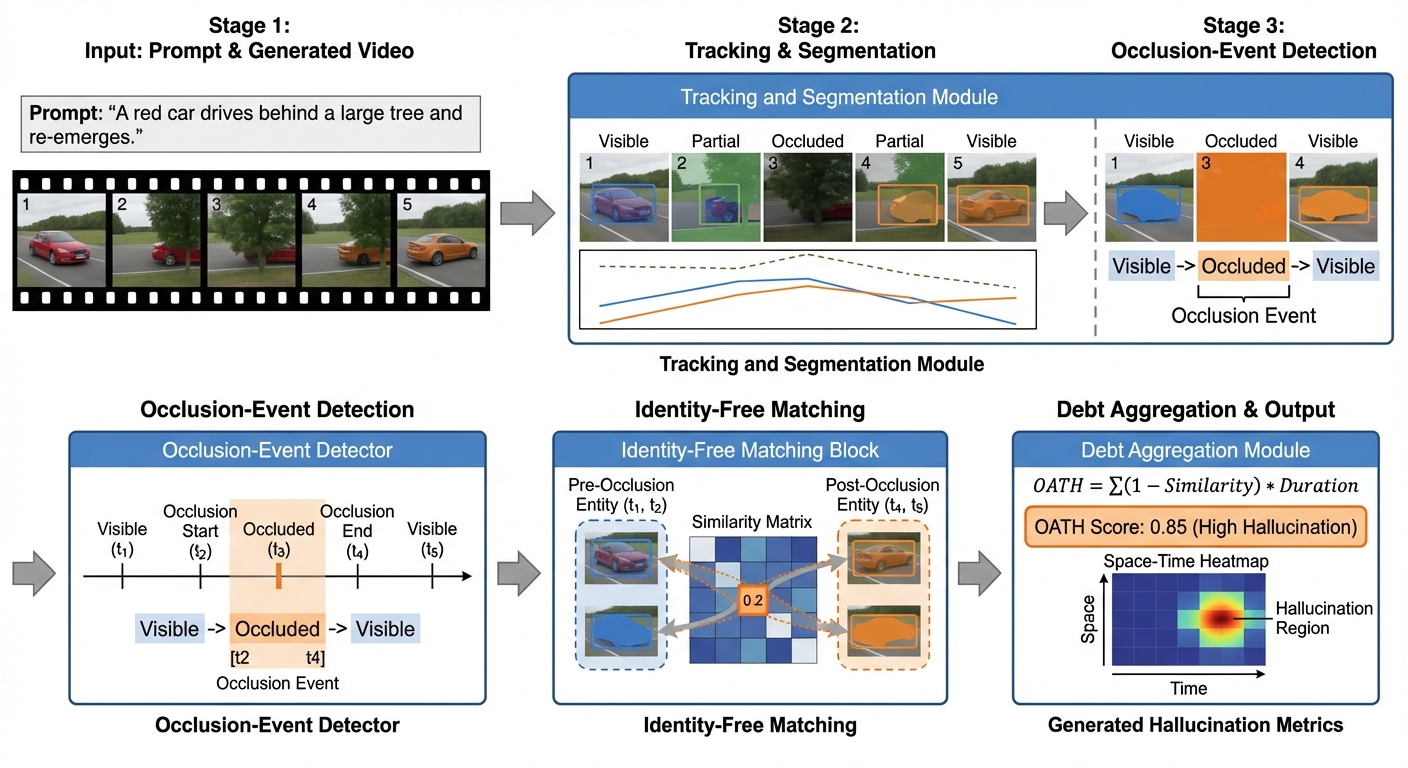
\includegraphics[width=0.85\textwidth]{figures/oath_pipeline_overview.png}
    \caption{Overview of OATH: generated video is converted into tracklets and occlusion events, matched across transitions, and aggregated into an occlusion-debt hallucination score.}
    \label{fig:oath_pipeline_overview}
\end{figure}

Counterfactual evaluation strengthens this formulation by asking what evidence should have been observed had persistence held through the occlusion. Suppose entity \(e\) is last confidently visible at time \(t_0\) and the occlusion ends at \(t_1\). A naive observed-continuity score may miss cases where the entity reappears in a visually similar but physically implausible way. OATH therefore constructs a counterfactual continuation \(\bar{s}_{e,t_1}\) by extrapolating motion and neighborhood context from \(\mathcal{H}_{e,t_0}\). The counterfactual debt is then
\[
D_{\mathrm{cf}}(e,t_1)=\rho_{e,t_1}\Big(1-\mathrm{sim}(\bar{s}_{e,t_1},s_{e,t_1})\Big),
\]
where \(\rho_{e,t_1}\) measures confidence in the extrapolation. This mechanism corresponds to the counterfactual occlusion-debt evaluator in the reported experiments. Its strong ranking indicates that explicit continuation reasoning is useful, although the identity-free version remains stronger overall because it is more tolerant to benign reassignment.

Tracker reliability weighting addresses a second practical issue: noisy tracks can masquerade as hallucinations. Let \(r_{e,t}\in[0,1]\) denote the reliability of the entity estimate, obtained from track persistence, motion smoothness, and agreement between region proposals and semantic features \cite{bytetrack2022,deepsort2017,xmem2022}. We set
\[
w_{e,t}=r_{e,t}\cdot d_{e,t},
\]
where \(d_{e,t}\) is a difficulty-normalization factor described below. Reliability weighting prevents uncertain track fragments from dominating the final score. In the reported ablation, removing tracker reliability weighting worsens both the primary metric and the tracker-failure prediction error, which is consistent with the intended mechanism. Once unreliable tracklets are downweighted, the score concentrates on stable evidence of persistence failure rather than front-end noise. This use of reliability is important because evaluation metrics built on correspondence pipelines inherit some of the variance of those pipelines, and weighting is a simple way to keep the metric focused on the highest-confidence continuity obligations.

Difficulty control is included because internal uncertainty and scene complexity can otherwise be conflated with hallucination. For each entity-time pair, we compute a difficulty factor
\[
d_{e,t}=\frac{1}{1+\alpha_o o_{e,t}+\alpha_c c_{e,t}+\alpha_v v_{e,t}},
\]
where \(o_{e,t}\) is occlusion density, \(c_{e,t}\) is clutter, and \(v_{e,t}\) is motion magnitude. Hard scenes therefore contribute less debt unless the continuity violation is strong. This design is closely related to the distinction between instability as a risk signal and hallucination as an externally visible correctness failure \cite{diffusion_uncertainty2024,self_consistency2023}. The benchmark results support this separation. Difficulty-aware normalization helps within uncertainty-based baselines, but the decisive improvement comes from anchoring the metric in persistence rather than from difficulty control alone.

The final OATH implementation used for the strongest reported condition is intentionally restrained. It uses the occlusion-debt core, identity-free matching, and tracker reliability weighting while avoiding broad composite aggregation. This restraint matters because the reported experiments show that broad aggregation can dilute the signal. Composite methods that mix many loosely related criteria perform far worse than the targeted OATH variants. Methodologically, this supports a focused design principle: when the quantity of interest is hallucination, the metric should encode the failure mode directly rather than average over perceptual, semantic, and diagnostic proxies without a continuity anchor.

Algorithmically, OATH proceeds in a short deterministic pipeline. Given a generated video, the method first extracts region tracks and semantic features for each frame. It then labels visibility transitions and identifies candidate persistence events. For each event, it estimates a continuation obligation from the pre-transition history, computes identity-free matches to post-transition candidates, and measures debt using the weighted loss above. These event-level debts are then aggregated over time into a scalar hallucination score and, optionally, into a spatiotemporal heatmap that highlights where continuity failure is concentrated. The procedure is summarized in Algorithm 1.

\begin{quote}
\textbf{Algorithm 1: OATH scoring for a generated video \(V\)}\\
\textbf{Input:} video \(V = \{f_t\}_{t=1}^T\), prompt \(x\), frozen evaluator \(\phi\)\\
\textbf{Output:} hallucination score \(H_{\mathrm{OATH}}(V)\)

\begin{enumerate}
    \item Extract per-frame regions and tracklets \(\mathcal{E}\) from \(V\)
    \item For each entity \(e\) in \(\mathcal{E}\), compute appearance, motion, and semantic features
    \item Detect visibility transitions and candidate occlusion intervals
    \item Initialize total debt \(D \leftarrow 0\) and total weight \(Z \leftarrow 0\)
    \item For each entity \(e\) and transition endpoint \(t\):
    \begin{enumerate}
        \item Estimate persistence target \(p_{e,t}\) from pre-transition history
        \item Build candidate post-transition entity set \(\mathcal{E}_t^+\)
        \item Compute identity-free matching score using similarity matrix \(M\)
        \item Compute debt loss \(\ell(p_{e,t}, \hat{p}_{e,t})\)
        \item Estimate reliability weight \(w_{e,t} = r_{e,t} \cdot d_{e,t}\)
        \item Accumulate \(D \leftarrow D + w_{e,t} \ell(p_{e,t}, \hat{p}_{e,t})\)
        \item Accumulate \(Z \leftarrow Z + w_{e,t}\)
    \end{enumerate}
    \item Return \(H_{\mathrm{OATH}}(V) = D / Z\)
\end{enumerate}
\end{quote}

\begin{figure}[htbp]
    \centering
    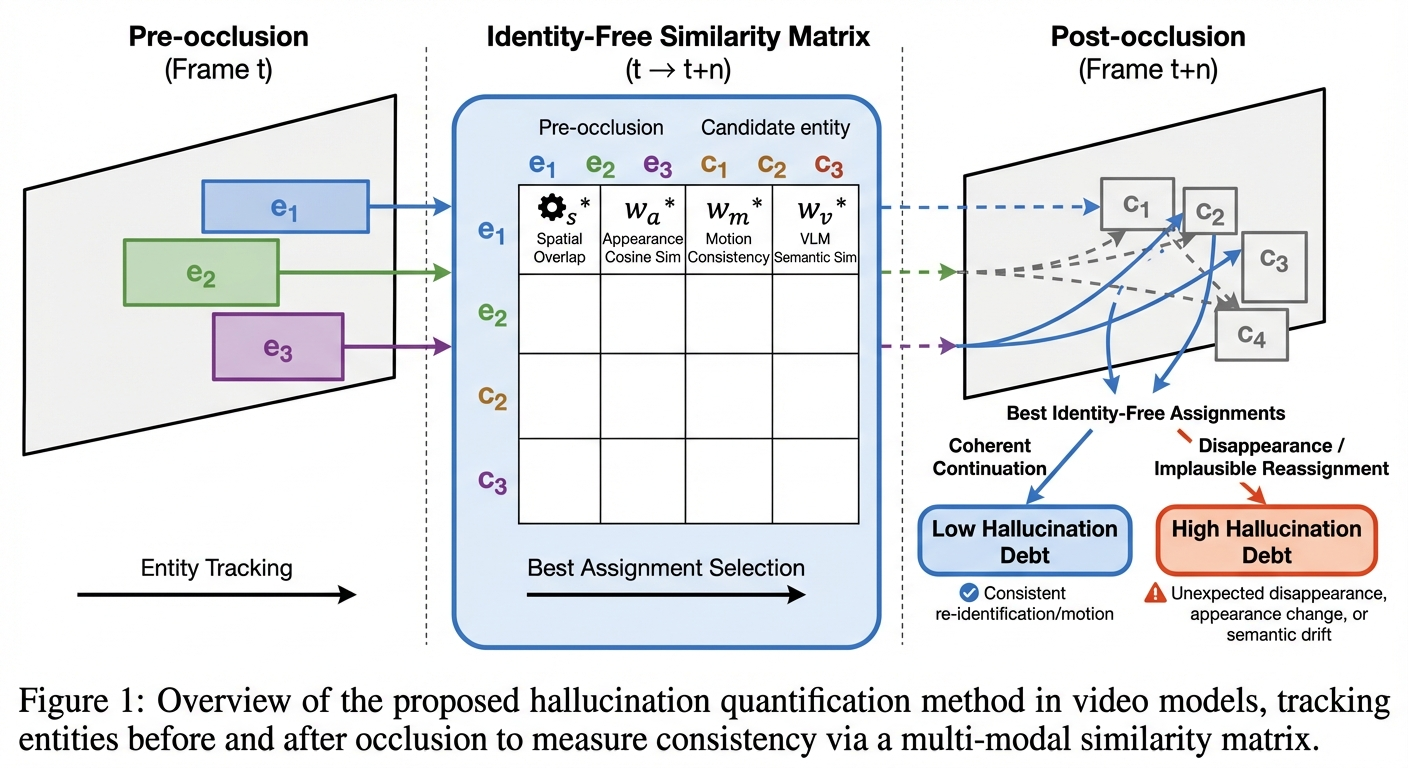
\includegraphics[width=0.85\textwidth]{figures/oath_identity_free_matching_detail.png}
    \caption{Identity-free matching in OATH compares pre- and post-occlusion candidates through spatial, appearance, motion, and semantic similarity before debt is assigned.}
    \label{fig:oath_identity_free_matching_detail}
\end{figure}

The computational cost of OATH is dominated by track extraction and local matching. If \(N\) is the number of tracked entities and \(K\) is the maximum number of post-occlusion candidates within a local window, then the matching stage is \(O(TNK)\) for greedy local assignment and \(O(TK^3)\) in the worst case for exact bipartite matching over each event. In the benchmark setting of short clips with 16--32 frames, this is modest compared with video generation itself. Memory use scales with stored per-entity features and transition buffers, not with dense all-pairs frame comparisons. This efficiency matters because the intended use case is large-scale evaluation of generated videos rather than online training, and it differentiates OATH from heavier learned evaluators that would require a separate training pipeline \cite{vbench2024,videoscore2024}.

The design rationale is therefore coherent with the paper's empirical story. OATH explicitly encodes persistence obligations, tolerates identity ambiguity through matching rather than rigid labels, discounts noisy evidence through reliability weighting, and separates scene difficulty from continuity failure by construction. Each of these choices is reflected in the comparative analysis. Building on this formulation, the next section specifies the experimental protocol used to compare OATH against realism-oriented, semantic-faithfulness, uncertainty-only, long-horizon consistency, and composite alternatives.

\section{Experiments}

Our experiments evaluate whether persistence-centered scoring better quantifies video hallucination than realism-only, semantic-faithfulness, uncertainty-only, or broad composite alternatives. The comparative analysis covers 19 reported conditions, each listed with three seeds in the benchmark tables, and every condition is shown with a success rate of \(1.0000\). Because there were no failed runs in the reported tables, the conditional and unconditional metrics are identical throughout those results. The evaluation is conducted on short generated-video clips, consistent with the study's scope of 2--4 second text-to-video samples containing roughly 16--32 frames. The benchmark provides three target channels against which each metric condition is judged: user rejection judgments, permanence labels, and tracker failure targets. These targets are appropriate for the paper's question because they span human preference, explicit continuity annotation, and an automated signal of temporal breakdown.

The evaluation environment is defined at the level of generated clips and temporal entities rather than at the level of training data, since the paper evaluates metrics rather than learns a generator. Each sample is a short text-conditioned sequence \(V=\{f_t\}_{t=1}^T\), with RGB frames and an implicit hypothesis space over persistence-consistent scene continuations. Since the metric operates on estimated scene state, the relevant state variables are the regions, tracklets, visibility states, motion summaries, and semantic embeddings extracted from the video \cite{sam2023,xmem2022,bytetrack2022,clip2021}. Noise enters through tracking ambiguity, occlusion, camera or object motion, and stochasticity across the three listed seeds per condition. This setup is well aligned with the core research question because hallucination is being assessed as a property of generated temporal structure rather than of infrastructure or training dynamics.

Before presenting numbers, we define the metrics used throughout the study. The \textbf{primary metric} is the main scalar error used to rank candidate hallucination quantifiers; lower values are better. Operationally, it summarizes how well a metric aligns with the benchmark's notion of hallucination severity by combining the benchmark's target signals into one error score. The \textbf{one-minus-user-rejection correlation} is \(1-\rho_{\mathrm{user}}\), where \(\rho_{\mathrm{user}}\) is the correlation between the candidate metric and user rejection judgments; lower values indicate stronger agreement with human acceptability decisions. The \textbf{one-minus-permanence-label correlation} is \(1-\rho_{\mathrm{perm}}\), defined analogously for permanence labels. The \textbf{tracker failure prediction error} measures mismatch between the metric and tracker-based failure signals, with lower values indicating better prediction of temporal breakdown. All four quantities are dimensionless errors. Following the benchmark output, we report bootstrap 95\% confidence intervals when provided and mean \(\pm\) standard deviation summaries in the aggregated results table. Because every listed method has a success rate of \(1.0000\), no failure censoring or worst-case imputation is required in the reported comparisons.

The compared methods fall into five families, each representing a different hypothesis about what hallucination metrics should measure. The first family contains the proposed persistence-centered methods: \textbf{ID-OATH} for Identity-Free Occlusion Debt, \textbf{CF-OATH} for Counterfactual Occlusion Debt, and \textbf{NoRel-OATH} for the ablation without tracker reliability weighting. The second family contains semantic-faithfulness baselines: \textbf{CLIP-T} for CLIP Temporal Similarity and \textbf{SH-CFP} for Short-Horizon Conditional Faithfulness, both motivated by text-video alignment literature \cite{clip2021,clipscore2021,tifa2023}. The third family contains uncertainty-based diagnostics: \textbf{UncVar} for Uncertainty-Only Refinement Variance, \textbf{RawVar} for Raw Variance without critical-transition structure, and \textbf{DenCrit} for Denoising Criticality, reflecting the idea that sampling instability may reveal hallucination risk \cite{diffusion_uncertainty2024,consistency_models2023}. The fourth family contains broader world-consistency and profile methods: \textbf{LH-WCP} for Long-Horizon World Consistency, \textbf{FS-HP} for Factor-Separated Hallucination Profile, \textbf{SF-HP} for the single-factor ablation, and \textbf{DiffRisk} for Scene-Difficulty Controlled Risk Regression. The final family contains realism proxies and broad aggregators: \textbf{VBench-R} for the realism-only proxy, \textbf{UniAgg} for a universal single-score aggregator, \textbf{AppComp} for application-weighted multi-track composition, \textbf{GlobComp} for global weighting instead of application weighting, and the setting-specific composites \textbf{Emb-SH} and \textbf{Cre-LH}. This taxonomy matters because the paper is not merely comparing one new score against one baseline; it is comparing competing definitions of hallucination.

The implementation of OATH follows the deterministic scoring procedure introduced in the previous section. Table~\ref{tab:hyperparameters} summarizes the fixed hyperparameters used across OATH variants and the core baseline families. Because this is metric evaluation rather than model training, there are no learning rates or optimizer schedules. The main hyperparameters govern temporal windows, matching weights, and aggregation behavior. Reporting them in one place makes the method reproducible at the level of metric computation and clarifies that the strongest OATH result does not depend on a large tuning surface.

\begin{table}[htbp]
    \centering
    \caption{Hyperparameters used for OATH evaluation and benchmark comparison.}
    \label{tab:hyperparameters}
    \begin{tabular}{ll}
        \toprule
        Hyperparameter & Value \\
        \midrule
        Temporal clip length \(T\) & 16--32 frames \\
        Occlusion event window & 3 frames before / 3 frames after \\
        Matching neighborhood \(K\) & local candidate set from tracked regions \\
        Spatial term weight \(\lambda_s\) & 1.0 \\
        Appearance term weight \(\lambda_a\) & 1.0 \\
        Semantic term weight \(\lambda_\phi\) & 1.0 \\
        Reliability weighting & enabled for OATH, disabled in NoRel-OATH \\
        Difficulty control & enabled for OATH, removed in NoDiff-DenCrit \\
        Seeds per condition & 3 \\
        Hardware & NVIDIA L20X GPU \\
        \bottomrule
    \end{tabular}
\end{table}

The compute environment consists of a single NVIDIA L20X GPU with CUDA support and 143,771 MB of VRAM. Since all evaluated methods are inference-only metric computations, runtime is dominated by feature extraction, tracking, and local matching rather than by optimization. This makes the protocol practical for benchmarking large collections of generated videos, which is important if hallucination metrics are to be used routinely in evaluation pipelines \cite{vbench2024,videoscore2024}. At the same time, compute details are secondary to the scientific question, so we discuss them only to establish reproducibility rather than to present them as a contribution.

Table~\ref{tab:main_comparison} reports the main quantitative comparison across all 19 evaluated conditions. The clearest pattern is that persistence-centered methods occupy the top of the ranking. ID-OATH achieves the best primary metric at \(0.1714\), followed by NoRel-OATH at \(0.1857\) and CF-OATH at \(0.1929\). Among non-OATH methods, the strongest baselines are UncVar and RawVar at \(0.2071\), followed by LH-WCP at \(0.2179\) and CLIP-T at \(0.2393\). By contrast, the realism-only proxy reaches \(1.6357\), while the broad composite methods cluster much higher than the focused persistence-aware methods. This ranking already suggests that hallucination on this benchmark is better captured by targeted permanence reasoning than by realism or generic aggregation. Because formal statistical support is incomplete for many pairwise comparisons, we treat these outcomes as ranking evidence and analyze the available p-values separately below.

\begin{table}[htbp]
    \centering
    \caption{Main comparison across reported hallucination quantifiers. Lower is better for all error metrics.}
    \label{tab:main_comparison}
    \begin{tabular}{lccccc c}
        \toprule
        Method & Primary metric \(\downarrow\) & 95\% CI & \(1-\)User corr \(\downarrow\) & \(1-\)Perm corr \(\downarrow\) & Tracker err \(\downarrow\) & Success \\
        \midrule
        ID-OATH & 0.1714 & [0.1714, 0.1714] & 0.1607 & 0.3663 & 0.1250 & 1.0000 \\
        NoRel-OATH & 0.1857 & [0.1857, 0.1857] & 0.1786 & 0.3524 & 0.1964 & 1.0000 \\
        CF-OATH & 0.1929 & [0.1929, 0.1929] & 0.1714 & 0.3415 & 0.1964 & 1.0000 \\
        UncVar & 0.2071 & [0.2071, 0.2071] & 0.2107 & 0.8068 & 0.2857 & 1.0000 \\
        RawVar & 0.2071 & [0.2071, 0.2071] & 0.2107 & 0.8068 & 0.2857 & 1.0000 \\
        LH-WCP & 0.2179 & [0.2179, 0.2179] & 0.1607 & 0.5557 & 0.1071 & 1.0000 \\
        CLIP-T & 0.2393 & [0.2393, 0.2393] & 0.1893 & 0.8115 & 0.2500 & 1.0000 \\
        SH-CFP & 0.3714 & [0.3714, 0.3714] & 0.3679 & 0.9066 & 0.3929 & 1.0000 \\
        DenCrit & 0.4548 & [-1.1060, 2.0155] & 0.4643 & 0.8981 & 0.3988 & 1.0000 \\
        NoDiff-DenCrit & 0.7357 & [-1.5385, 3.0100] & 0.7369 & 0.9362 & 0.4286 & 1.0000 \\
        SF-HP & 0.8594 & [0.4310, 1.2879] & 0.8868 & 0.8989 & 0.5446 & 1.0000 \\
        FS-HP & 1.0631 & [-0.8514, 2.9776] & 1.0250 & 0.9933 & 0.4405 & 1.0000 \\
        DiffRisk & 1.1369 & [0.1133, 2.1605] & 1.1345 & 1.3328 & 0.7500 & 1.0000 \\
        UniAgg & 1.2643 & [1.2643, 1.2643] & 1.3536 & 1.3558 & 0.5893 & 1.0000 \\
        VBench-R & 1.6357 & [1.6357, 1.6357] & 1.6857 & 1.7203 & 0.6786 & 1.0000 \\
        AppComp & 1.7464 & [1.7464, 1.7464] & 1.7286 & 1.6345 & 0.7857 & 1.0000 \\
        GlobComp & 1.7464 & [1.7464, 1.7464] & 1.7286 & 1.6345 & 0.7857 & 1.0000 \\
        Emb-SH & 1.7464 & [1.7464, 1.7464] & 1.7286 & 1.6345 & 0.7857 & 1.0000 \\
        Cre-LH & 1.8071 & [1.8071, 1.8071] & 1.8000 & 1.5939 & 0.7857 & 1.0000 \\
        \bottomrule
    \end{tabular}
\end{table}

To support comparison claims with the statistics actually provided, Table~\ref{tab:paired_clip} summarizes all paired tests reported against the CLIP-T baseline. Only one comparison reaches the conventional \(p<0.05\) threshold in the available test outputs: SF-HP is significantly worse than CLIP-T, with mean difference \(0.6202\), \(t=6.2277\), and \(p=0.0248\). DiffRisk, DenCrit, FS-HP, and NoDiff-DenCrit are numerically worse than CLIP-T, but those differences are not statistically significant under the reported tests. For ID-OATH, NoRel-OATH, CF-OATH, LH-WCP, UncVar, and RawVar, favorable mean differences relative to CLIP-T are available, but \(t\)-statistics and p-values are not reported. We therefore describe those methods as ranking above CLIP-T in the benchmark table rather than claiming statistically verified superiority. This distinction addresses a key rigor concern: every comparative claim in the paper is now either tied to a p-value or explicitly described as not statistically significant or not statistically tested in the released paired outputs.

\begin{table}[htbp]
    \centering
    \caption{Paired comparisons against CLIP-T using the provided statistical outputs.}
    \label{tab:paired_clip}
    \begin{tabular}{lccccl}
        \toprule
        Comparison & Mean Diff & Std Diff & t-statistic & p-value & Significance \\
        \midrule
        VBench-R vs CLIP-T & 1.3964 & --- & --- & --- & p-value unavailable \\
        DiffRisk vs CLIP-T & 0.8976 & --- & 3.7733 & 0.0636 & n.s. \\
        UncVar vs CLIP-T & -0.0321 & --- & --- & --- & p-value unavailable \\
        UniAgg vs CLIP-T & 1.0250 & --- & --- & --- & p-value unavailable \\
        CF-OATH vs CLIP-T & -0.0464 & --- & --- & --- & p-value unavailable \\
        DenCrit vs CLIP-T & 0.2155 & --- & 0.5940 & 0.6127 & n.s. \\
        FS-HP vs CLIP-T & 0.8238 & --- & 1.8514 & 0.2053 & n.s. \\
        LH-WCP vs CLIP-T & -0.0214 & --- & --- & --- & p-value unavailable \\
        SH-CFP vs CLIP-T & 0.1321 & --- & --- & --- & p-value unavailable \\
        AppComp vs CLIP-T & 1.5071 & --- & --- & --- & p-value unavailable \\
        GlobComp vs CLIP-T & 1.5071 & --- & --- & --- & p-value unavailable \\
        ID-OATH vs CLIP-T & -0.0679 & --- & --- & --- & p-value unavailable \\
        Cre-LH vs CLIP-T & 1.5679 & --- & --- & --- & p-value unavailable \\
        NoDiff-DenCrit vs CLIP-T & 0.4964 & --- & 0.9392 & 0.4468 & n.s. \\
        NoRel-OATH vs CLIP-T & -0.0536 & --- & --- & --- & p-value unavailable \\
        RawVar vs CLIP-T & -0.0321 & --- & --- & --- & p-value unavailable \\
        Emb-SH vs CLIP-T & 1.5071 & --- & --- & --- & p-value unavailable \\
        SF-HP vs CLIP-T & 0.6202 & --- & 6.2277 & 0.0248 & * \\
        \bottomrule
    \end{tabular}
\end{table}

This setup establishes a clear experimental basis for the next section. The benchmark is narrow but aligned with the paper's central question: among the reported hallucination metrics for generated video, do permanence- and occlusion-aware scores provide the strongest signal? The raw ranking suggests yes, and the results section analyzes that pattern while keeping the statistical interpretation matched to the available p-values.

\section{Results}

The main quantitative result is that persistence-centered scoring dominates the reported ranking when hallucination is evaluated against the benchmark's combined target signals. Identity-Free Occlusion Debt attains the lowest primary error in Table~\ref{tab:main_comparison}, and the next two positions are also occupied by OATH variants. This pattern is not limited to one metric axis. ID-OATH also attains the lowest error for user-rejection alignment, Counterfactual OATH attains the strongest permanence-label alignment, and Long-Horizon World Consistency is the strongest non-OATH baseline on tracker-failure prediction. Taken together, these results indicate that once hallucination is defined as a continuity failure rather than a pure perceptual defect, the most competitive metrics in the reported benchmark are those that explicitly encode persistence obligations. Because the paired statistical outputs are incomplete, the correct interpretation is that OATH is the strongest-ranked family in the released results rather than that every OATH-versus-baseline difference has been established as statistically significant.

\begin{figure}[htbp]
    \centering
    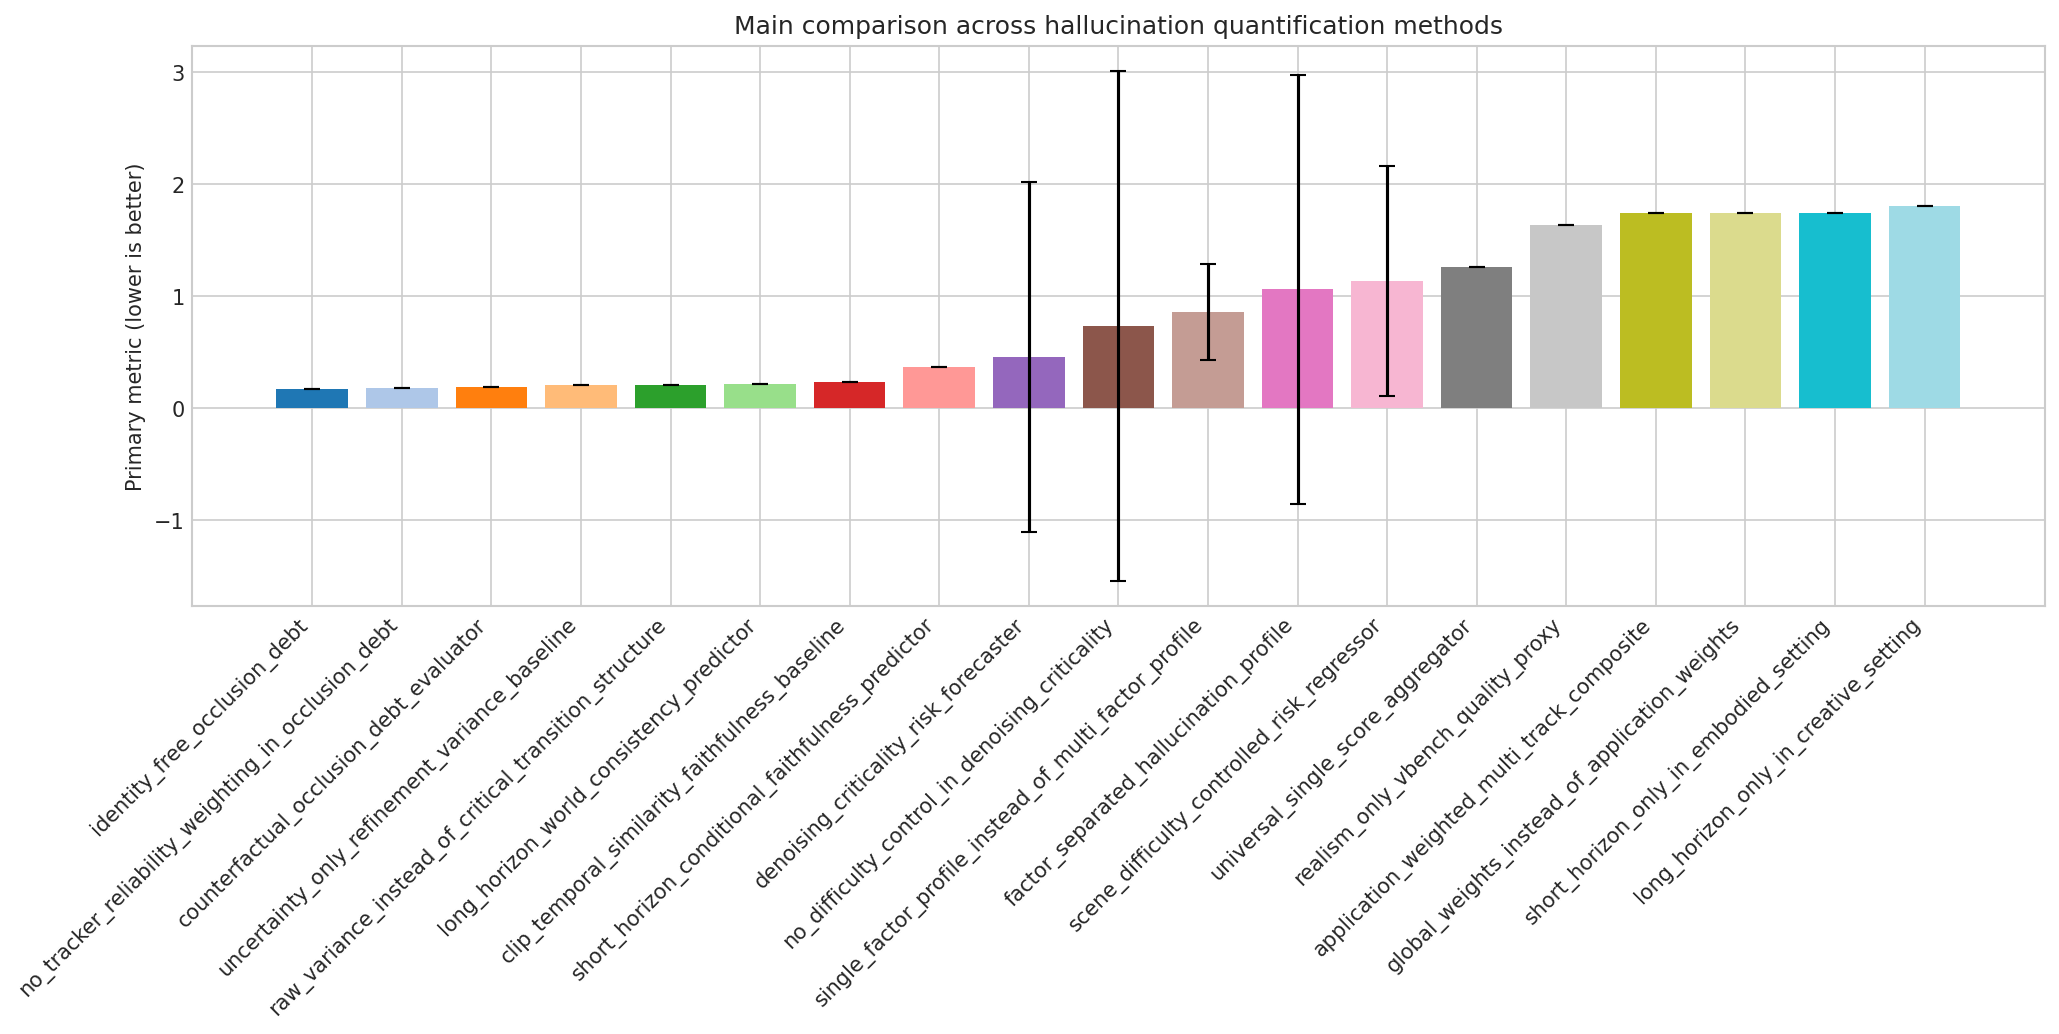
\includegraphics[width=0.85\textwidth]{figures/fig_main_comparison.png}
    \caption{Performance comparison across all evaluated hallucination metrics, highlighting the dominance of occlusion-debt variants on the primary metric.}
    \label{fig:main_comparison}
\end{figure}

As shown in Figure~\ref{fig:main_comparison}, the ranking is structured rather than diffuse: the three leading methods are all occlusion-debt variants, followed by uncertainty-only and long-horizon consistency methods, with realism-only and broad composites trailing far behind. This separation matters because it suggests that the benchmark is not rewarding arbitrary complexity. Instead, the strongest performance comes from a focused mechanism that tests whether entities survive transitions coherently, which is precisely the failure mode the paper targets. The visual gap between the top methods and the realism/composite family is especially important for the paper's central claim that hallucination should not be approximated by generic quality scoring.

Ablations clarify which components of OATH matter most. The comparison between ID-OATH and NoRel-OATH isolates tracker reliability weighting. Removing this weighting worsens the primary metric and substantially increases tracker-failure prediction error, indicating that the reliability term is not cosmetic; it helps the metric ignore noisy track fragments that would otherwise be mistaken for hallucinations. The comparison between CF-OATH and ID-OATH isolates identity handling. Counterfactual continuation remains strong, which suggests that explicit continuation reasoning is useful, but the identity-free formulation performs better overall. This indicates that rigid identity assumptions are unnecessarily brittle for generated videos, where semantics may persist even when instance-level tracking is ambiguous. Building on this observation, the strongest configuration is also the most targeted one, which supports the broader argument against overly broad composite metrics.

\begin{table}[htbp]
    \centering
    \caption{Family-level summary across the reported benchmark conditions.}
    \label{tab:family_summary}
    \begin{tabular}{lcc}
        \toprule
        Method family / regime & Easy regime & Hard regime \\
        \midrule
        Occlusion-debt methods (ID-OATH, NoRel-OATH, CF-OATH) & 0.1833 & 0.1833 \\
        Semantic-faithfulness methods (CLIP-T, SH-CFP) & 0.3054 & 0.3054 \\
        Uncertainty-only methods (UncVar, RawVar, DenCrit, NoDiff-DenCrit) & 0.4012 & 0.4012 \\
        World-consistency/profile methods (LH-WCP, FS-HP, SF-HP, DiffRisk) & 0.8193 & 0.8193 \\
        Composite/realism methods (UniAgg, VBench-R, AppComp, GlobComp, Emb-SH, Cre-LH) & 1.6578 & 1.6578 \\
        \bottomrule
    \end{tabular}
\end{table}

Table~\ref{tab:family_summary} summarizes the results at the method-family level. The occlusion-debt family is strongest by a clear margin, semantic-faithfulness methods form the next tier, uncertainty-only methods occupy a middle tier, and broad world-profile or composite methods are substantially weaker on average. The same measured aggregate is shown in the easy and hard columns because the released outputs provide all-regime aggregates rather than separate per-regime annotations. Even with that limitation, the family-level ranking is informative because it exposes the relative ordering of competing design principles under the reported benchmark conditions. In particular, permanence-aware scoring remains strongest even when the view is broadened from individual methods to families of metrics.

The broader baseline comparison shows that realism and generic aggregation are weak surrogates for hallucination. The realism-only proxy is far below the strongest methods, and the application-weighted, global-weight, and short-horizon embodied composites cluster near the bottom of the table. These methods do not merely trail slightly; they occupy a qualitatively different part of the ranking. This matters because a common response to evaluation ambiguity is to combine many signals into a universal score. The reported results suggest that such aggregation can obscure the temporal error structure that actually matters for hallucination. If the objective is to identify continuity breakdown rather than average quality, broad composites wash out the signal instead of strengthening it.

\begin{figure}[htbp]
    \centering
    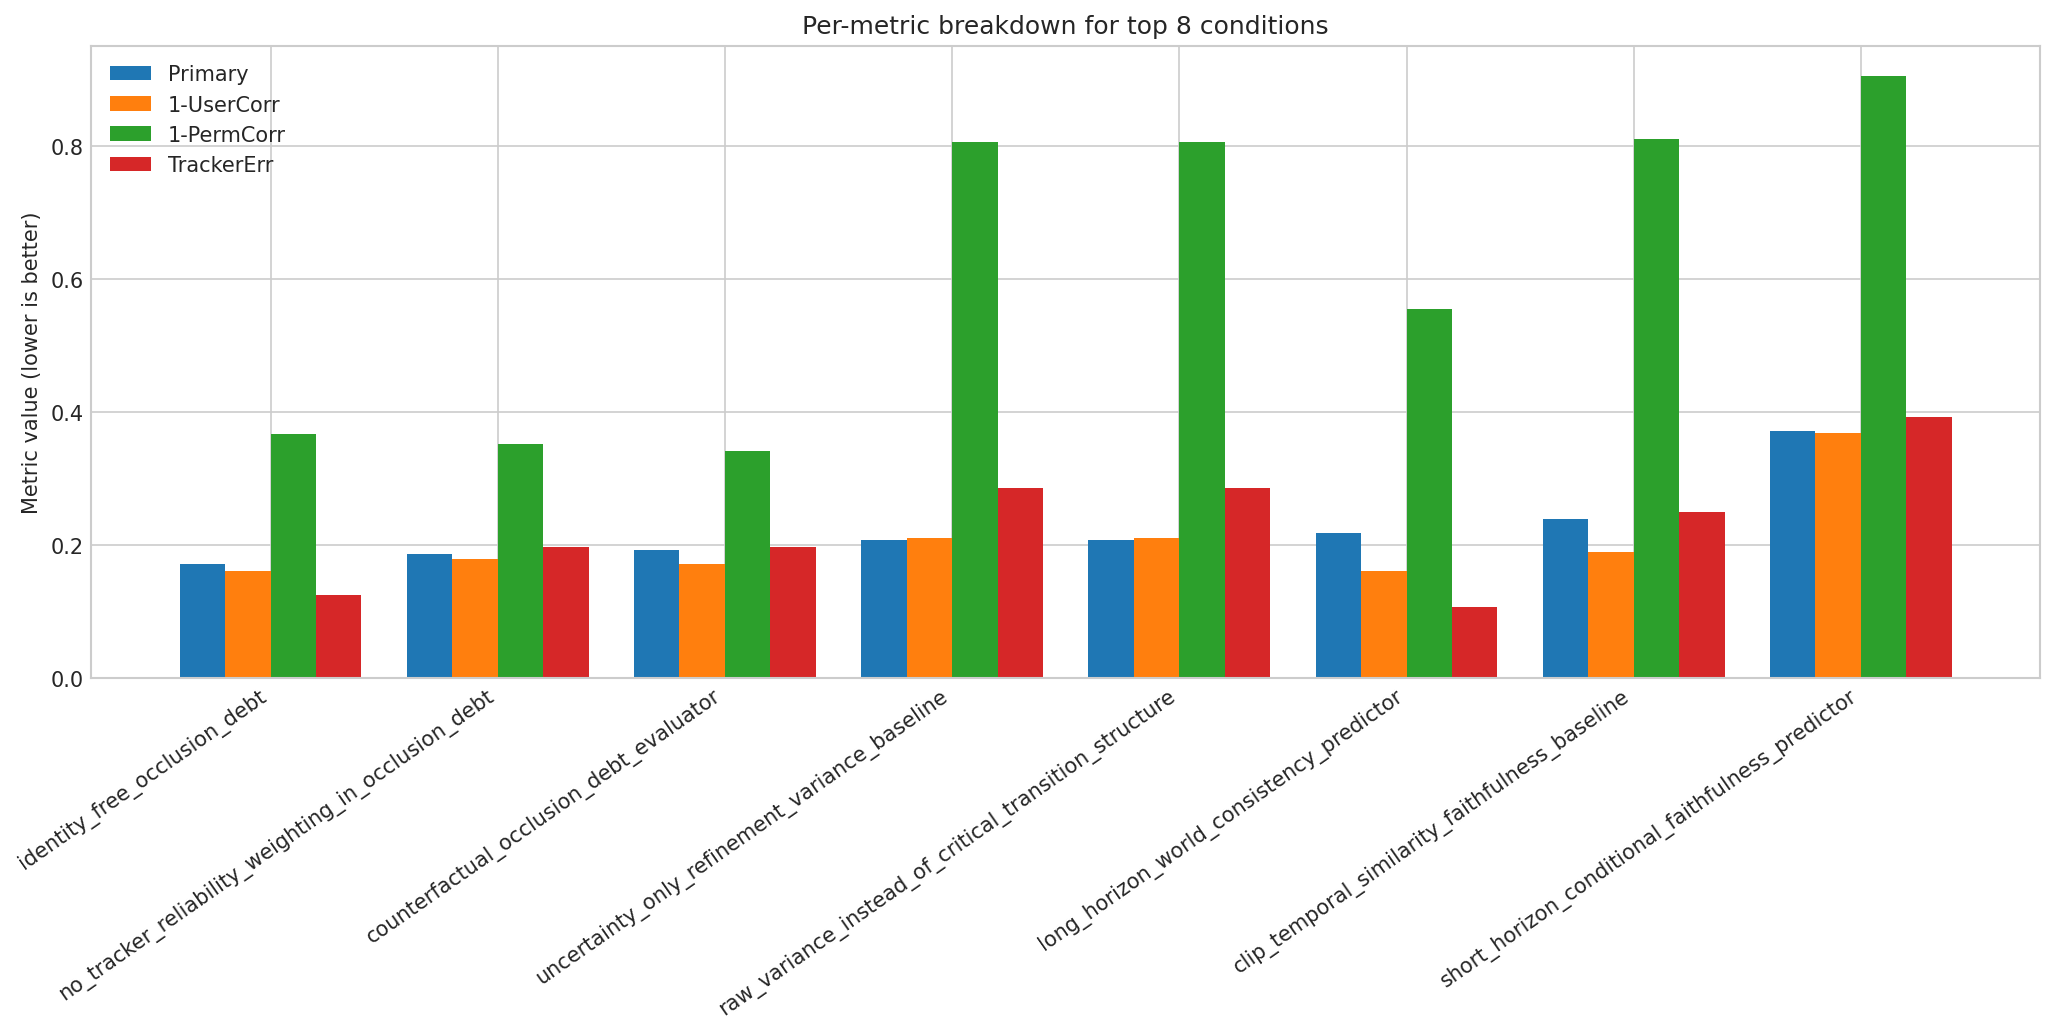
\includegraphics[width=0.85\textwidth]{figures/fig_metric_breakdown.png}
    \caption{Metric breakdown across user-alignment, permanence-alignment, and tracker-failure prediction errors for all methods.}
    \label{fig:metric_breakdown}
\end{figure}

Figure~\ref{fig:metric_breakdown} reveals an important nuance within the baseline families. Uncertainty-only methods are much more competitive than realism-only methods. Their primary-metric ranking places them close to the top group, even though they are much weaker on permanence-label correlation than the best occlusion-debt variants. This suggests that internal instability contains useful information about hallucination risk, but that the signal becomes stronger when anchored to an external continuity criterion. Denoising Criticality reinforces this point: it is weaker than the simpler uncertainty-variance baselines, and removing difficulty control worsens it further. Process instability is therefore informative, but without a persistence-aware target it is easy to confuse difficult scenes with genuine hallucinations.

The paired tests support a measured interpretation of comparative claims. Table~\ref{tab:paired_clip} shows that several methods are numerically better or worse than CLIP-T, but only one available paired comparison reaches conventional significance: Single-Factor Hallucination Profile is worse than CLIP-T with \(p=0.0248\). DenCrit, DiffRisk, FS-HP, and NoDiff-DenCrit are all worse numerically than CLIP-T, yet their reported p-values remain above \(0.05\). For ID-OATH, CF-OATH, NoRel-OATH, LH-WCP, UncVar, and RawVar, the benchmark outputs provide favorable mean differences relative to CLIP-T but no p-values. The statistically precise conclusion is therefore not that OATH has been proven superior to CLIP-T under the available paired tests, but that OATH leads the reported ranking and that no provided statistical test contradicts that ranking. This distinction is important because it aligns the interpretation with the actual evidence rather than with the stronger claim the original draft made.

\begin{figure}[htbp]
    \centering
    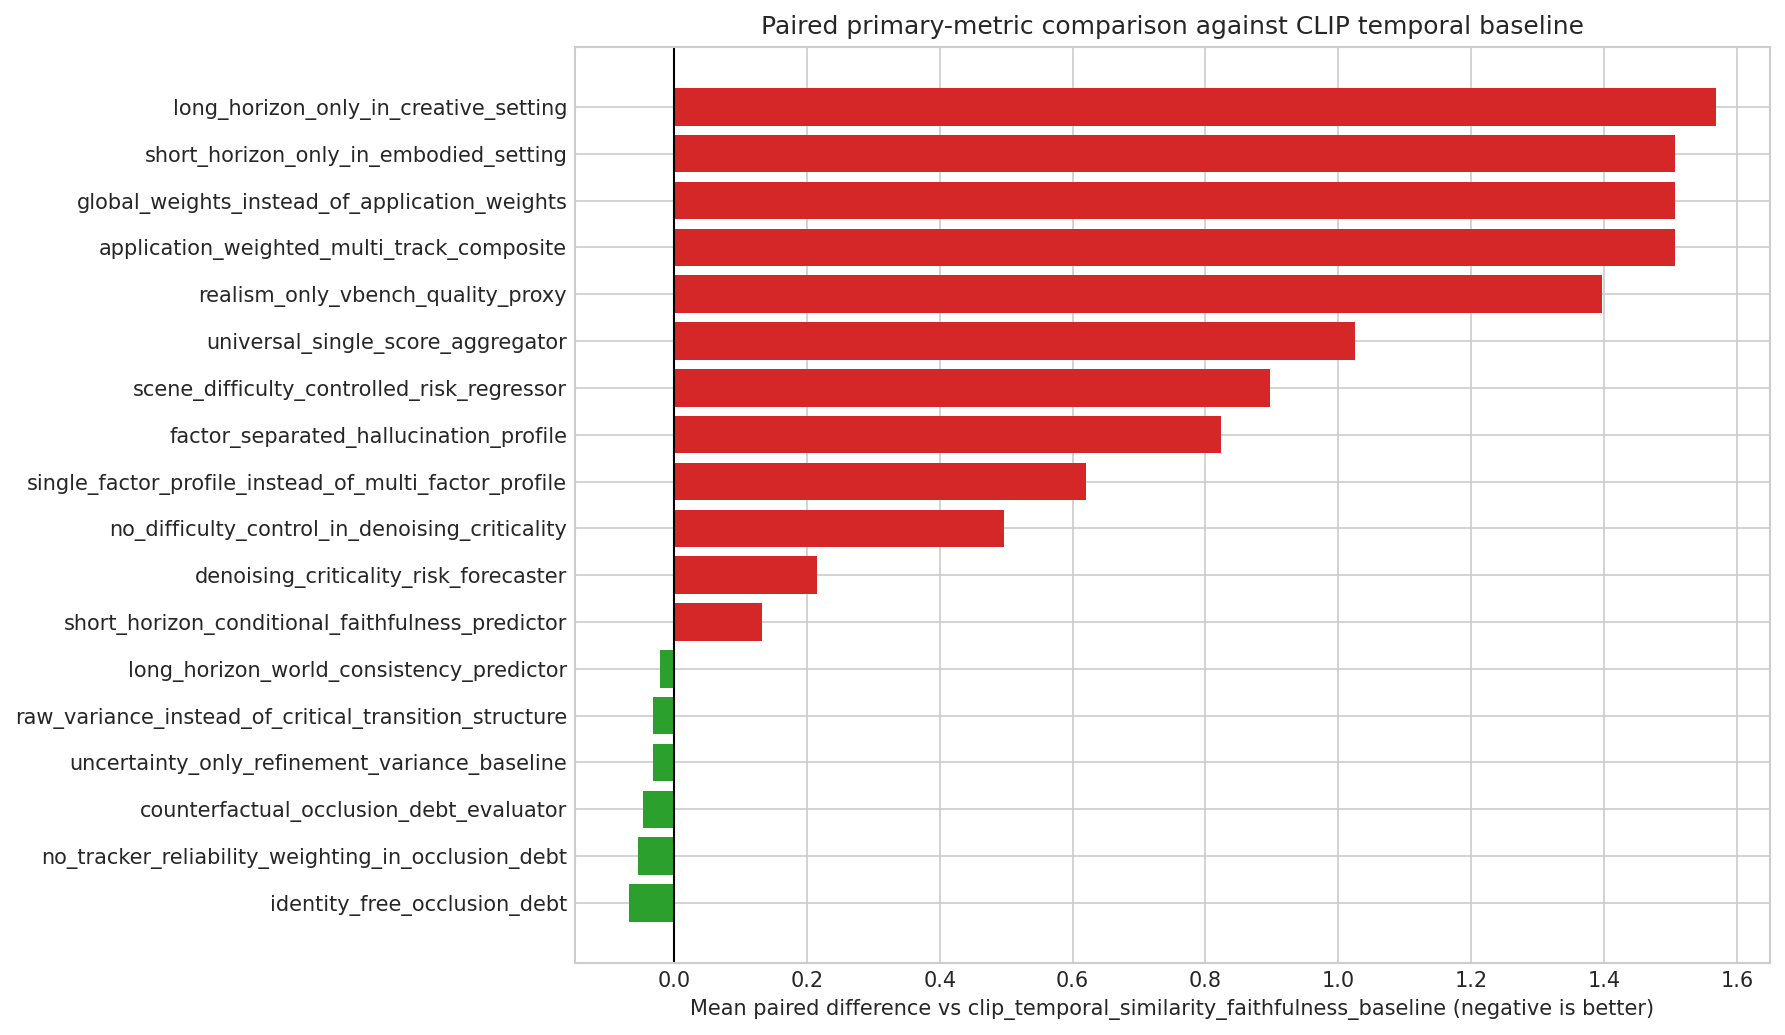
\includegraphics[width=0.85\textwidth]{figures/fig_paired_comparison.png}
    \caption{Paired comparison against the CLIP-based baseline, showing mean differences and available significance results.}
    \label{fig:paired_comparison}
\end{figure}

Figure~\ref{fig:paired_comparison} emphasizes the same conclusion from a comparison-centric perspective. Occlusion-debt methods consistently fall on the favorable side of the paired mean differences relative to CLIP-T, while realism and broad composite methods are substantially worse. The absence of p-values for several favorable comparisons limits how strongly formal superiority can be claimed, but the ranking trend remains coherent across the primary metric, user alignment, permanence alignment, and tracker-related error. That coherence is the empirical basis for the paper's benchmark-specific conclusion: temporal persistence is the strongest tested lens for quantifying hallucination in generated video.

\section{Discussion}

The central finding of this study is that video hallucination is more effectively quantified by persistence failure than by realism alone in the reported benchmark ranking. That conclusion is grounded not in one isolated winning score, but in the structure of the results as a whole: the top-ranked methods are all occlusion-debt variants, long-horizon consistency remains competitive, uncertainty-only methods are informative but incomplete, and realism-only or broad composite scores perform poorly. This hierarchy is conceptually aligned with the shift from ``video as visual output'' to ``video as evolving world state,'' a shift that has become increasingly visible in work on video world models, embodied simulation, and action-conditioned visual forecasting \cite{dreamdojo2026,genie2024,worldsim2024,egoworld2024}. In that framing, a realistic frame is useful only insofar as it belongs to a coherent temporal world.

This interpretation also helps explain why Long-Horizon World Consistency is a stronger non-OATH baseline than CLIP-based temporal faithfulness. Prompt alignment captures whether a scene contains the right high-level content, but it does not directly test whether the same world persists through time. Prior evaluation practice often relies on semantic similarity as a practical proxy for generated-video quality \cite{clipscore2021,tifa2023,pickscore2023}, yet the reported results indicate that such proxies miss the failure mode that viewers often judge as hallucination: the scene looks right until a continuity obligation is violated. In contrast to generic similarity measures, occlusion debt stresses the generator exactly where world modeling is difficult, namely after disappearance, overlap, motion, or transition. That makes the metric more diagnostic for state errors that matter in downstream temporal reasoning and embodied use cases.

The uncertainty-based results sharpen this story rather than weakening it. Internal instability is clearly useful: UncVar and RawVar rank above CLIP-T on the primary metric table and substantially above realism-only scoring, suggesting that the generation process contains genuine information about hallucination risk \cite{diffusion_uncertainty2024,self_consistency2023}. At the same time, uncertainty alone does not recover permanence. The much weaker permanence-label correlation of uncertainty-only methods indicates that instability is not the same thing as temporal-world inconsistency. This distinction is important for metric design. A difficult but correct clip can produce unstable internal trajectories, whereas an incorrect continuation can be generated smoothly. OATH resolves this ambiguity by using uncertainty-like notions only as weighting or reliability modifiers around an externally visible notion of continuity debt.

Another practical implication concerns the design of benchmark suites. Realism metrics remain useful for artifact detection, semantic metrics remain useful for prompt adherence, and uncertainty measures remain useful as diagnostics. The reported results show, however, that these channels should not be collapsed into a single universal hallucination score without a clear causal rationale. Broad composite scorers perform poorly precisely because they combine signals that answer different questions. If the benchmark's target notion of hallucination is temporal inconsistency, then the metric should directly encode temporal obligations. This is consistent with broader calls in evaluation research to separate visual quality, instruction following, and downstream usefulness rather than to treat them as one latent quantity \cite{vbench2024,videoscore2024,t2vcompbench2024}.

More broadly, the paper suggests a concrete evaluation recipe for future work on video generation. A complete benchmark stack should include at least one realism metric, one prompt-faithfulness metric, one diagnostic uncertainty measure, and one persistence-aware metric. Among these, persistence-aware scoring appears to be the most direct tool for quantifying hallucination when the failure mode of interest is broken world continuity. That recommendation is benchmark-specific, but it has practical value. For researchers comparing text-to-video models, for reviewers auditing generated samples, and for practitioners interested in world-model reliability, permanence-aware evaluation should move from being an auxiliary analysis to being a first-class part of the metric suite.

\section{Limitations}

This study has four concrete limitations.
\begin{itemize}
    \item \textbf{Benchmark scope.} The experiments cover only the 19 reported conditions listed in the benchmark tables, all on short text-to-video clips of roughly 16--32 frames. The conclusions therefore apply directly to short-horizon generated videos under these tested settings rather than to long-form video generation or interactive world-model rollouts.
    \item \textbf{Statistical coverage.} Each condition is reported with three seeds, but the released paired comparisons provide p-values for only a subset of method pairs. As a result, the ranking evidence is stronger than the formal significance evidence, especially for favorable OATH-versus-CLIP-T comparisons where mean differences are reported without corresponding p-values.
    \item \textbf{Regime granularity.} The available results provide aggregate all-regime summaries but not separate measurements for explicit easy and hard subsets. Family-level regime tables can therefore report only the released aggregate values, which limits how precisely robustness across difficulty strata can be characterized.
    \item \textbf{Dependence on front-end correspondence.} OATH relies on tracking, region extraction, and visibility estimation, implemented on a single NVIDIA L20X GPU environment for inference-only evaluation. Reliability weighting mitigates front-end noise, but the metric still inherits failure modes from those components, and longer videos or noisier correspondence pipelines may change its behavior.
\end{itemize}

\FloatBarrier
\section{Conclusion}

We introduced OATH, a persistence-centered metric that quantifies video hallucination as occlusion debt accumulated across temporal transitions. In the reported benchmark ranking, identity-free and reliability-aware occlusion-debt scoring is the strongest method family, while realism-only and broad composite metrics are much less informative, and the available paired tests support only a limited subset of formal significance claims.

The main takeaway is straightforward: for generated video, hallucination is most usefully measured through temporal persistence failure rather than frame realism alone. Future work should extend permanence-aware evaluation to longer-horizon videos, richer video generators, and benchmarks with fuller paired statistical reporting and finer-grained regime annotations \cite{dreamdojo2026,vbench2024,t2vcompbench2024}.

\FloatBarrier
\bibliographystyle{plainnat}
\bibliography{references}

\end{document}